\svnid{$Id: digging_deeper.tex 80911 2026-04-14 12:40:55Z jagers $}

\chapter{Digging deeper} \label{Chp:DiggingDeeper}
At the end of the `Getting started' chapter, we shortly introduced the slider in the lower left corner of each plot and indicated that it can be used to select other time steps and other spatial co-ordinates.
This chapter describes how to

\begin{itemize}
\item combine plots (\Sref{Sec:AddToPlot}),
\item looking at result differences (\Sref{Sec:DiffFiles}),
\item use the Plot Manager (\Sref{Sec:PlotManager}),
\item use the slider (\Sref{Sec:InteractPlot}),
\item create animations (\Sref{Sec:AnimateResults}),
\item define your own derived variables (\Sref{Sec:DefVariables}),
\item define your own colour maps (\Sref{Sec:DefColourMap}),
\item use the Grid selection window (\Sref{Sec:GridView}), and
\item use command logging to create macros (\Sref{Sec:Macros}).
\end{itemize}

\section{Setting preferences} \label{Sec:Preferences}
From the File menu of the main \QUICKPLOT\ window, select the option Preferences...~ .
This will open the preferences dialog which has eight sections.

\begin{figure}[H]
\center{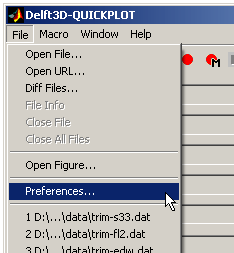
\includegraphics[width=50mm]{Ch05/open_preferences.png}}
\caption{Start the preferences dialog.}
\label{fig:5.1}
\end{figure}

\subsection{General preferences} \label{Sec:GenPrefs}
This section allows you to select the characteristics of the font used in all dialogs (excluding menus) of \QUICKPLOT.
This functionality is mainly intended for cases in which the default system font selection is unsuitable; the user interface does not scale with font size changes.
The second item, the work directory, is for information only.
It shows where the files are located that the program is running.
This refers to the source folder when running within MATLAB.
The \QUICKPLOT\ binary is a self-extractor that unpacks upon first use in a temporary folder; the work directory listed here tells you where those files are located.
The organization name can be set; this name is only used in the default figure templates (see \Sref{Sec:PlotManager}).
Some data files contain time zone information.
By default, \QUICKPLOT\ ignores this information, but it can also perform time zone conversions while processing the data.
\QUICKPLOT\ depends on GhostScript for writing pdf-files with page labels (see \Sref{Sec:print_figures}); if \QUICKPLOT\ cannot locate GhostScript, you can specify the location here.
Finally, there is a switch to display the \QUICKPLOT\ version number in the title bar of the main window.
This is mainly useful when you have different \QUICKPLOT\ versions open for comparison.

\begin{figure}[H]
\center{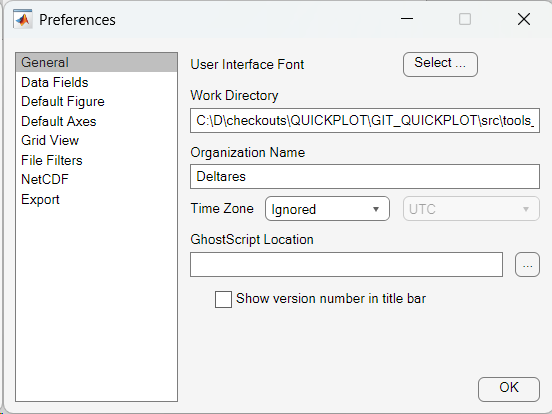
\includegraphics[width=100mm]{Ch05/prefs_general.png}}
\caption{General section of the preferences dialog.}
\label{fig:GeneralPrefs}
\end{figure}

\subsection{Data Fields preferences} \label{Sec:DataFieldsPrefs}
The Data Fields section allows you to set some settings for working with data fields.
Currently the only option is a choice for sorting station names.
By default the order of the stations matches the order of the stations in the data file ("No Sorting").
You can choose to sort the station names lexicographically (numbers are ordered as characters, so \keyw{10} is ordered between \keyw{1} and \keyw{2}) or alphanumerically (numbers are sorted numerically, characters alphabetically).

\begin{Remark}
\item A change in the station sort order affects all files opened after changing the setting.
The setting doesn't change upon reloading the data file, but it does update when closing the file and reopening it.
\end{Remark}

\begin{figure}[H]
\center{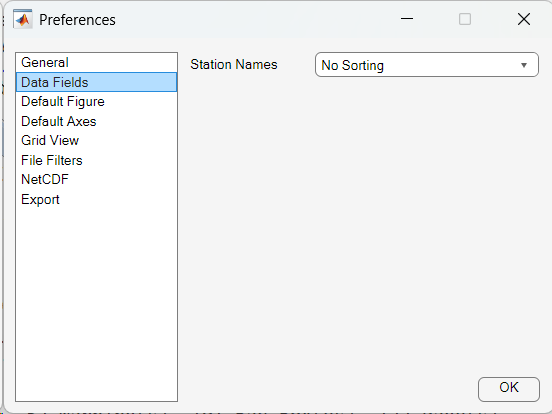
\includegraphics[width=100mm]{Ch05/prefs_datafields.png}}
\caption{Data Fields section of the preferences dialog.}
\label{fig:DataFieldPrefs}
\end{figure}

\subsection{Default Figure preferences} \label{Sec:FigurePrefs}
The Default Figure section allows you to personalize a number of figure settings.
It allows you to change the figure colours.
Instead of the simple default figure, it is also possible to point to a previously saved figure file.
\QUICKPLOT\ will use the layout of the selected figure each time you press Quick View.
If the figure file contains multiple axes, the Quick View plot action will use the front axes.
The second step is to determine where the figure should open on the screen.
You can choose the exact position, but the primary choice is which screen to use in a multi-screen set-up.
The final choices let you choose the default setting for graphics rendering (using OpenGL is typically the best option) and for graphics smoothing (switched off by default for reasons of speed and consistency).

\begin{figure}[H]
\center{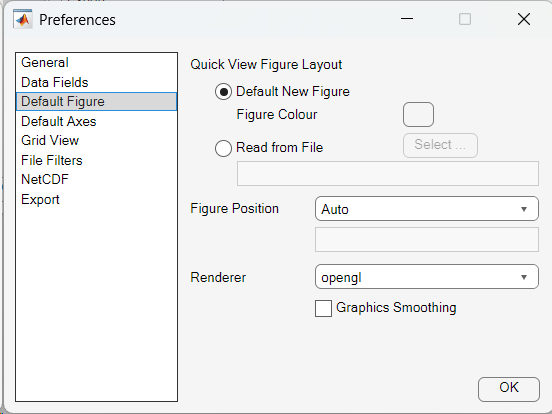
\includegraphics[width=100mm]{Ch05/prefs_figure.png}}
\caption{Default Figure section of the preferences dialog.}
\label{fig:FigurePrefs}
\end{figure}

\subsection{Default Axes preferences} \label{Sec:AxesPrefs}
The Default Axes section allows you to personalize a number of axes settings.
It allows you to change the axes colours and you can switch whether the bounding box of the axes are closed or that, as is the default, only the left and bottom axes are drawn.

\begin{figure}[H]
\center{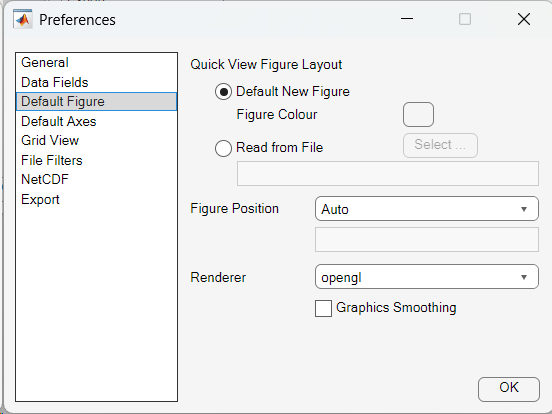
\includegraphics[width=100mm]{Ch05/prefs_figure.png}}
\caption{Default Axes section of the preferences dialog.}
\label{fig:AxesPrefs}
\end{figure}

\subsection{Grid View preferences} \label{Sec:GridViewPrefs}
The Grid View section allows you to change the colours used by the Grid View interface (see \Sref{Sec:GridView}) and to select whether grid indices should be drawn for curvilinear grids by the Grid View interface.
Switching of the drawing of grid indices may speed up the Grid View interface in case of large models.

\begin{figure}[H]
\center{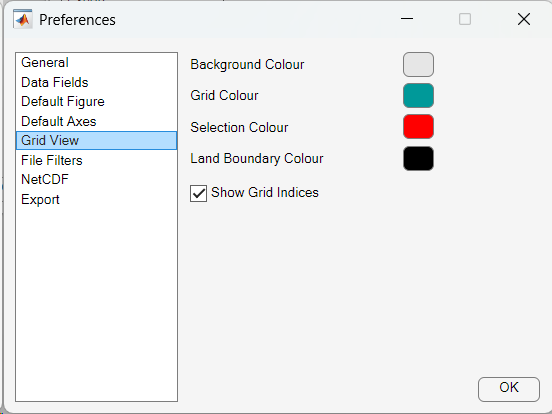
\includegraphics[width=100mm]{Ch05/prefs_gridview.png}}
\caption{Grid View section of the preferences dialog.}
\label{fig:GridViewPrefs}
\end{figure}

\subsection{File Filter preferences} \label{Sec:FileFilterPrefs}
The number of file filters that is available in the File Open dialog is limited.
The File Filter section allows you select the 15 file types that you use most often.
One entry is reserved for the file filter associated with type of the last opened file.
Note that \QUICKPLOT\ will try all file formats independent of the selected file filter, so the choice here is for your convenience of filtering long lists of files only.

\begin{figure}[H]
\center{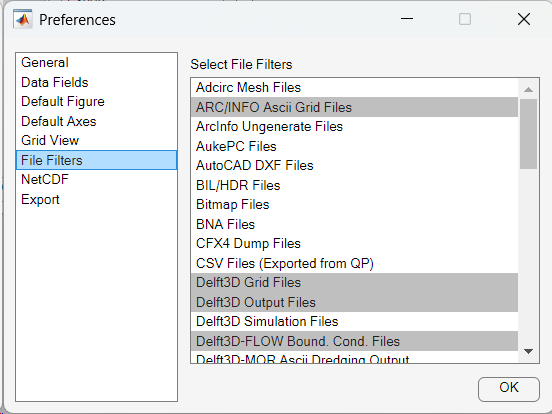
\includegraphics[width=100mm]{Ch05/prefs_filefilters.png}}
\caption{File Filters section of the preferences dialog.}
\label{fig:FileFiltersPrefs}
\end{figure}

\subsection{NetCDF preferences} \label{Sec:NetCDFPrefs}
Here you can make choices related to the netCDF file format.
Currently, there is only one choice, namely the way in which \QUICKPLOT\ processes netCDF \keyw{\_FillValue} keywords.
The netCDF conventions (sometimes referred to as the "NetCDF User Group (NUG)" conventions) state:

\begin{quote}
If neither \keyw{valid\_min}, \keyw{valid\_max} nor \keyw{valid\_range} is defined then generic applications should define a valid range as follows.
If the data type is byte and \keyw{\_FillValue} is not explicitly defined, then the valid range should include all possible values.
Otherwise, the valid range should exclude the \keyw{\_FillValue} (whether defined explicitly or by default) as follows.
If the \keyw{\_FillValue} is positive then it defines a valid maximum, otherwise it defines a valid minimum.
For integer types, there should be a difference of 1 between the \keyw{\_FillValue} and this valid minimum or maximum.
For floating point types, the difference should be twice the minimum possible (1 in the least significant bit) to allow for rounding error.
\footnote{\url{https://docs.unidata.ucar.edu/netcdf-c/current/attribute_conventions.html}}
\end{quote}

By default, \QUICKPLOT\ follows this rule, but at Delares the value of \num{-999} is often used as missing value, which based on the above-mentioned conventions gives a \keyw{valid\_range} that includes all positive values and only negative values down to \num{-999}.
However, this value may be within coordinate ranges, depth or elevation ranges, or in discharge ranges.

\begin{figure}[H]
\center{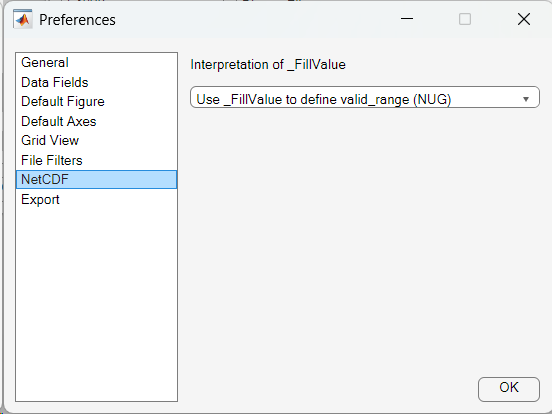
\includegraphics[width=100mm]{Ch05/prefs_netcdf.png}}
\caption{NetCDF section of the preferences dialog.}
\label{fig:NetCDFPrefs}
\end{figure}

\subsection{Export preferences} \label{Sec:ExportPrefs}
Here you can make choices related to data export.
You set the upper limit for the maximum number of time steps to be processed at once during a data export.
A larger value requires more internal memory.
The default is set to 10 has been selected for stability reasons; it should run fine on all systems.

\begin{figure}[H]
\center{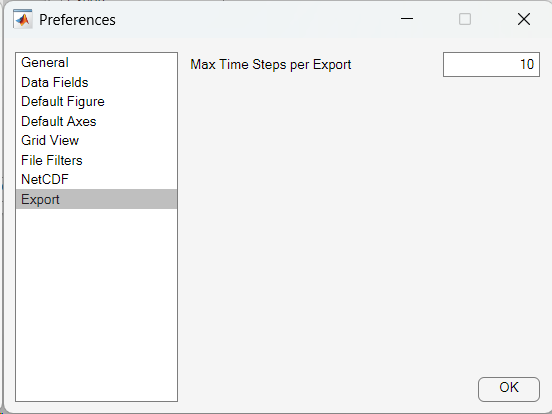
\includegraphics[width=100mm]{Ch05/prefs_export.png}}
\caption{Export section of the preferences dialog.}
\label{fig:ExportPrefs}
\end{figure}

\section{Combining multiple data sets in one plot} \label{Sec:AddToPlot}
In most cases it will be sufficient to plot only one quantity in a plot.
However, under certain circumstances you may want to combine two different variables or variables from different files in one plot.
Therefore, an `Add to Plot' button has been added next to the `Quick View' button.
By default the `Add to Plot' function adds the plot of the selected variable to the last created figure/axes using `Quick View'.
If you want to add a variable to another axes, you should use the Plot Manager to select the desired axes (see \Sref{Sec:PlotManager}).

The text on the `Add to Plot' button will turn red if the program detects some incompatibilities in the plot settings.
These checks currently include a check on dimensionality of the data set (e.g.\ trying to add a 2D spatial data set to a time-series plot) and a check on units (e.g.\ a velocity magnitude [m/s] cannot be added to a water level [m] plot, nor should a water level in [m] be added to a plot of water levels in [ft]).
Although the text turns red to warn you of such conflicts, the button will still works such that you can still combine data sets in one plot.

\begin{figure}
\center{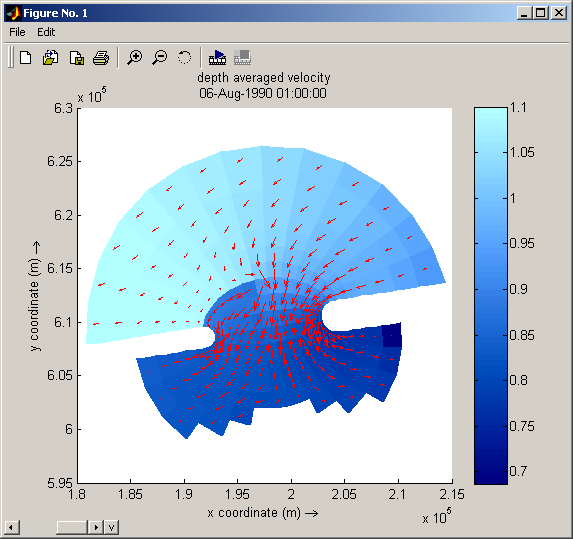
\includegraphics[width=100mm]{Ch05/water_level_patches_vectors.png}}
\caption{Overlay plot of the water level using patches and the depth averaged velocity using red vectors.}
\label{fig:5.5}
\end{figure}

\begin{Remark}
\item It is not possible to combine two plots with different colour maps in one figure.
\item It is not possible to combine two plots with different colour scaling in one axes.
\item It is not possible to combine plots with the presentation type set to continuous shades with other plot types, such as contours and vectors.
\end{Remark}

\subsection{Adding GIS layers} \label{Sec:GISLayer}
There are three methods by which you can add GIS data to figures.
\begin{enumerate}
\item Opening the GIS data just like any other data file, and adding quantities contained in it to the figure via the `Add to Plot' button.
Data stored in BNA File (\Autoref{Sec:FileBNA}) or ESRI shape File (\Autoref{Sec:FileSHP}) can be added in this way.
\item If the visualized data has global co-ordinates (longitude and latitude) then you can add via the Plot Manager (\Autoref{Sec:PlotManager}) a series of global data sets to the figure.
The options include: vector shorelines, country boundaries, and rivers from the Global Self-consistent, Hierarchical, High-resolution Geography (GSHHG) Database to the figure, and Web Map Service (WMS) data from NASA blue marble, Bing maps virtual earth, ESRI world imagery, and Open Street Map.
These options are unfortunately not available if other spatial co-ordinates are used.
\item An alternative option is store create an image (bitmap) of the desired background map via another tool, and to load the image file (\Autoref{Sec:FileBMP}).
The $x$ and $y$ co-ordinates of the lowerleft-corner as well as the width and height in $x$ and $y$ co-ordinates can be specified via the `File Options' dialog.
Note that the co-ordinates in the image must align with the co-ordinate using the figure since the image will not be warped (or than horizontal and vertical stretching) when it's added to the figure.
\end{enumerate}

\section{Difference of Files} \label{Sec:DiffFiles}

\begin{figure}[b]
\center{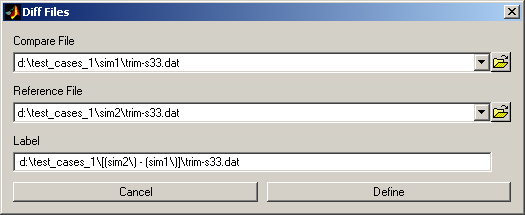
\includegraphics[width=\textwidth]{Ch05/diff_files.png}}
\caption{Diff Files dialog.}
\label{fig:difffiles}
\end{figure}

Often you will run multiple simulations to study the effect of certain parameter settings, change in forcing conditions or minor geometry changes.
If the effect is (initially) small, it may sometimes be difficult to spot the essence of the differences between two simulations.
The option to define and combine variables (described in \Sref{Sec:DefVariables}) allows you to define and subtract individual variables to look at the net effect of a model input change.
However, this method is quite laborous and error prone if you want to look at the differences of multiple quantities (possibly in multiple files).
The option to use logfiles (see \Sref{Sec:Macros}) to repeat some steps helps but is not always straightforward to use.
For this reason we have added a new feature called `Diff Files' to quickly subtract the contents of two data files.
The new option is available from the \menu{File} menu.
When you select the menu item, you will see the dialog shown in \Fref{fig:difffiles}.
The list boxes are automatically populated with the files already opened in the main dialog, but you can open additional files if needed (note: these additional files won't show up in the main dialog).
The algorithm will look for all quantities with identical names and identical time and space dimensions and subtract (on demand) the values in the second file from the values in the first file.
The last line of the dialog allows you to specify the name that should identify the difference of the files in the listbox in the main dialog.
In the main dialog you will subsequently be able to select of which quantity you would like to see the differences as shown in \Fref{fig:difffiles-example}.

\begin{Remark}
\item When looking at differences, please check the limits of vertical axes and color bars carefully.
If the differences are small and irregular they may very well result from numerical noise in the computations.
\item Since the algorithm checks for identical time and space dimensions, the differencing will fail if you change the number of output stations or the number of time steps.
Supporting such changes is considered for a future release.
\item The algorithm doesn't check for location or time changes, i.e.\ if you change grid, output times, or output stations (or reorder them) while keeping the grid dimensions, number of time steps and number of output stations identical then the `Diff Files' option will allow you to subtract the data from the original simulation.
The graphs will show you the location and times of the original (top) simulation.
\end{Remark}

\begin{figure}
\center{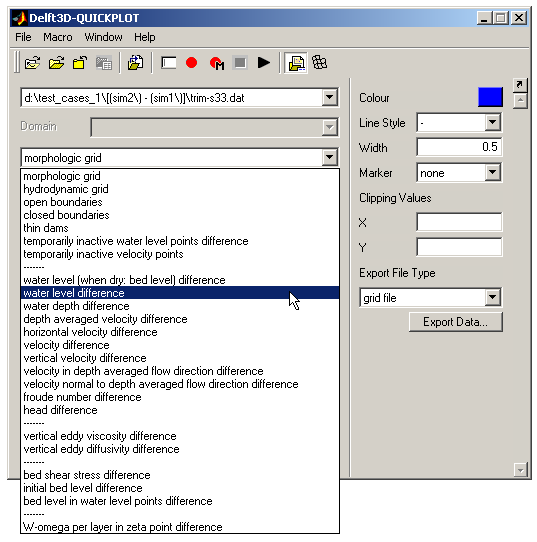
\includegraphics[width=0.8\textwidth]{Ch05/diff_files_example.png}}
\caption{Diff Files dialog.}
\label{fig:difffiles-example}
\end{figure}


\section{Plot Manager} \label{Sec:PlotManager}
If you want to add a variable to another plot than the last one created or if you want to delete a quantity from a plot, you should use the Plot Manager.
The Plot Manager can be opened from the Window menu in the main program window or by clicking on the button in the toolbar.


\begin{figure}
\center{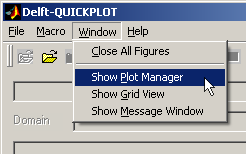
\includegraphics{Ch05/5-2a.png}
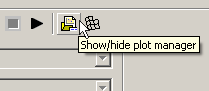
\includegraphics{Ch05/5-2b.png}}
\caption{Activation of the Plot Manager from the Window menu of the main program window.}
\label{fig:5.6}
\end{figure}


\begin{figure}
\center{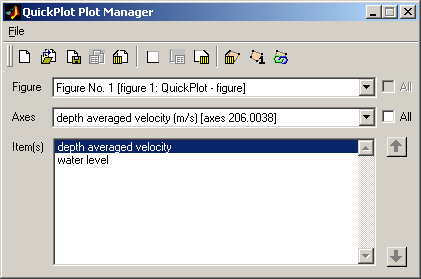
\includegraphics{Ch05/5-3a.png}}
\caption{Interface of the Plot Manager.}
\label{fig:5.7}
\end{figure}

The Plot Manager has a toolbar with buttons for

\begin{itemize}
\item creating new figures (some standard paper layouts are provided) and opening previously saved figures, saving figures, setting figure options (not yet available), deleting figures;
\item creating new axes, setting axes options (not yet available) and deleting axes;
\item deleting items (in axes), requesting information on items, and linking items for animations.
\end{itemize}

The selection boxes for figures and axes allow you to select all figures and axes.
The list box shows the names of the items in the selected axes (which may be located in multiple figures).
If the bare names of the items are the same, the names are automatically extended with the name of the file, selected time steps and M, N or K indices, and plot type if one or more of these labels will help to distinguish between the items.
More detailed information (in particular plot characteristics) for the selected item can be obtained by clicking the item information button in the toolbar.
Multiple items across multiple axes or even figures can be linked to animate or to scroll through at once.

The new figure button allows you to create a new figure with a standard layout.
\Fref{fig:5.8} shows a couple of standard layouts available.
All plots except for the free format figure contain the standard Deltares border.
You can edit all texts in the border by selecting the Edit Border option from the Edit menu in the figure (see Figures \ref{fig:5.9} and \ref{fig:5.10}).
More flexibility in figure layouts can be achieved making your own set of standard plot layouts and by using the load figure option instead of the new figure option.

\begin{figure}
\center{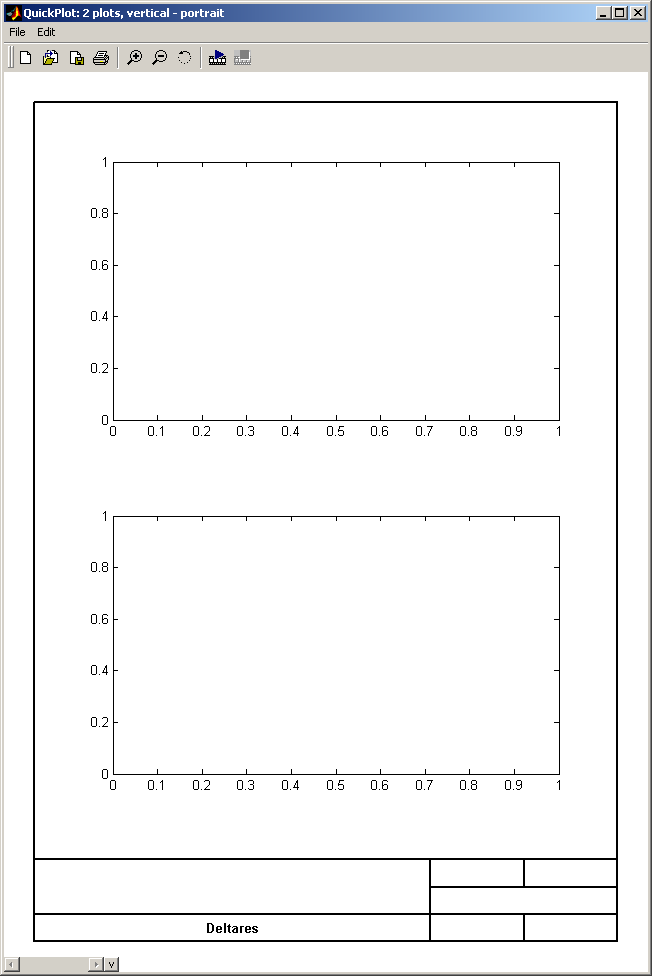
\includegraphics[width=100mm]{Ch05/2_plots_vertical_portrait.png}}
\caption{A couple of standard figure layouts created using the new figure button of the Plot Manager: 1 plot -- portrait, 2 plots, vertical -- portrait, 4 plots, 2x2 -- portrait, 2 plots, horizontal -- landscape.}
\label{fig:5.8}
\end{figure}

\begin{figure}
\center{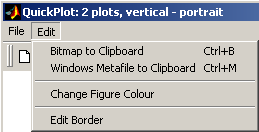
\includegraphics{Ch05/edit_border_select.png}}
\caption{Select Edit Border from the Edit menu to edit the border texts.}
\label{fig:5.9}
\end{figure}

\begin{figure}
\center{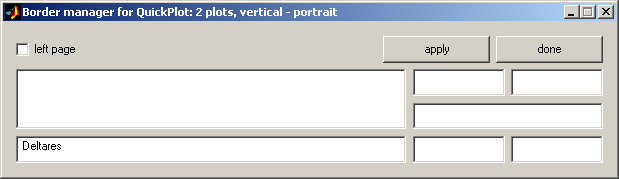
\includegraphics[width=100mm]{Ch05/edit_border_edit.png}}
\caption{The layout of the editor for the border texts matches the layout of the boxes.}
\label{fig:5.10}
\end{figure}

Furthermore, you can add axes to and remove axes from the selected figure using the next row of buttons.
There are three options for adding axes:

\begin{itemize}
\item one plot.
In this case one big axes is created (identical to the default axes that appears when pressing Quick View).
\item user selected subplot.
In this case a number of plots can be created based on a regular grid as illustrated by Figures \ref{fig:5.11} and \ref{fig:5.12}.
Note that the plots are numbered row-wise starting in the upper-left corner.
\item user positioned subplot.
In this case, you are asked to interactively draw the location of the axes in the figure.
The axes labels extend outside the indicated area.
\end{itemize}

\begin{figure}
\center{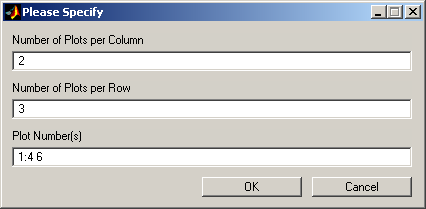
\includegraphics{Ch05/5-4.png}}
\caption{Dialog for defining five `user selected subplots' based on a regular grid of 3 plots on a row and 2 plots above each other.
All plots are created except plot number 5 (see \Fref{fig:5.12}).}
\label{fig:5.11}
\end{figure}

\begin{figure}
\center{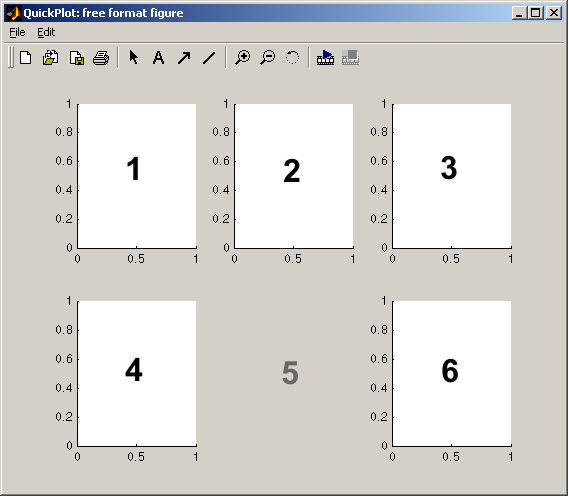
\includegraphics{Ch05/5-5.png}}
\caption{Five `user defined subplots' with an indication of their row-wise numbering.}
\label{fig:5.12}
\end{figure}

\begin{figure}
\center{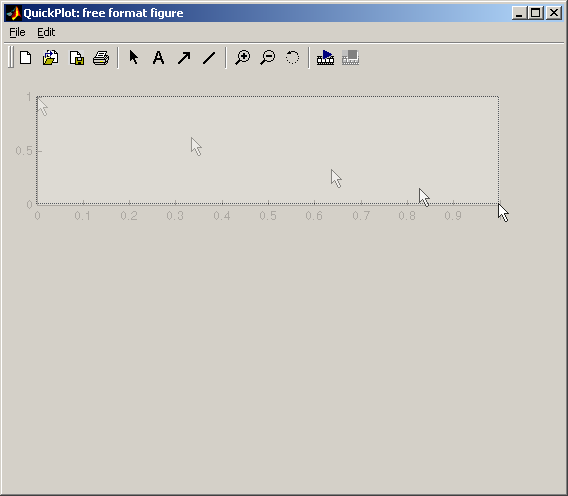
\includegraphics{Ch05/5-6.png}}
\caption{Example of the interactive positioning of a `user positioned subplot'.}
\label{fig:5.13}
\end{figure}

If you want to add a plot to a certain axes, select the figure to which the axes belong from the list of figures and, subsequently, select the axes from the list of axes.
Now, the desired axes are active and you can use the Add to Plot option to add a dataset to the active axes.
The lower listbox in the Plot Manager lists all items/quantities plotted in the axes (or if you check the `all' checkbox to the right of the axes listbox, all items in the current figure are listed).
You can select and delete some of them and you can link them for an animation (see also Sections \ref{Sec:InteractPlot} (interacting with plots) and \ref{Sec:AnimateResults} (animating results).

\section{Interacting with plots} \label{Sec:InteractPlot}
Where you can find the buttons for interacting with plots depends on the MATLAB version being used.
You may either find a toolbar with seven buttons as shown in \Fref{fig:5.14} or you may find only the left four buttons in the toolbar and the rest popping up in the upper right corner of the axes (see the right side of \Fref{fig:5.15}).
Let us first take a closer look at these functionalities... from left to right they provide the following functionality: create a new figure, load a figure from file, save a figure to file, print a figure (Windows only), zooming in, zooming out and rotating the plot.

\begin{figure}
\center{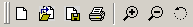
\includegraphics{Ch05/5-7.png}}
\caption{Toolbar buttons of a \QUICKPLOT\ figure.}
\label{fig:5.14}
\end{figure}

A zoom action should always start inside the plot area of the axes.
It works by dragging a zoom area with the left mouse button pressed down.
When the zoom-in mode is activated, you can zoom out with a right click.
When the zoom-out mode is activated, you can zoom out with the left button (single click) and zoom in with the right button (drag zoom area).
It is only possible to zoom out up to the dimensions of the original plot.
The rotation option is not relevant for most plots.
\QUICKPLOT\ only supports 3D plots for a few cases, such as for structured model output when using presentation type continuous shades, 3D particle tracks from \DPART\ and vector plots of the 3D velocity fields.
In such cases the rotation functionality can be useful.
Rotate the axes by pressing and holding down the left mouse button.
Typically the vertical scale needs to be exaggerated by at least a factor of 30; you can set the vertical scale via the axes properties in the Plot Manager (see \Autoref{Sec:PlotManager}).
When zooming in on a rotated plot, use single clicks only; do not drag a zoom window.

\begin{figure}
\center{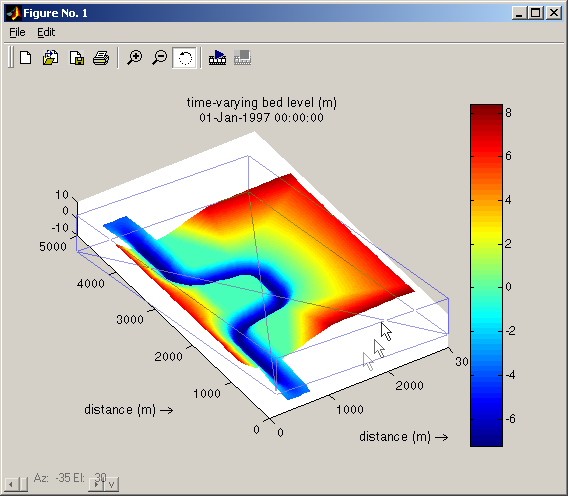
\includegraphics[width=70mm]{Ch05/5-8.png}
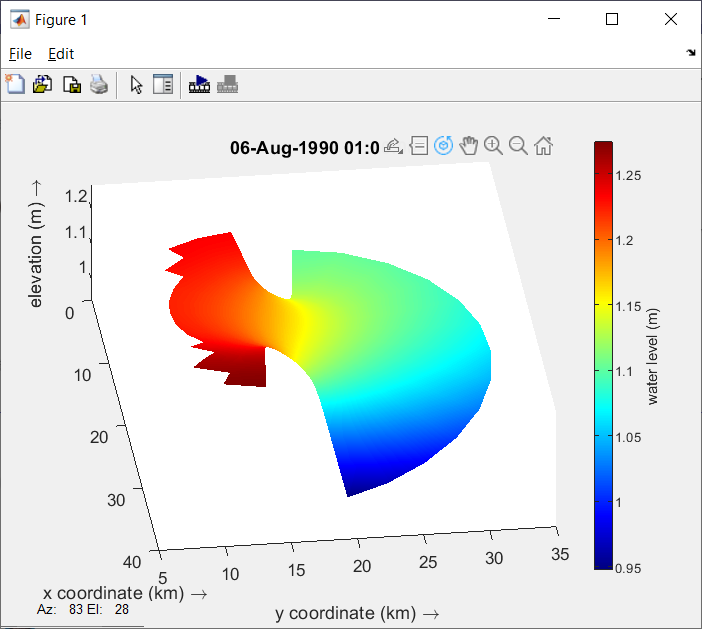
\includegraphics[width=70mm]{Ch05/rotate_2023a.png}}
\caption{Rotating a 3D topography (left: old MATLAB, right: recent MATLAB).}
\label{fig:5.15}
\end{figure}

A slider is drawn in the lower left corner of the plot window.
The slider can be used to change the time step, station or M, N, K co-ordinate of one or more of the objects in the plot.
The currently selected time step, station or M, N, K co-ordinate is shown in the tooltip of the slider.

To the right of the slider, there is a small button marked with the character v; that button, allows you to select the object and dimension (i.e., time step, station, M, N, or K co-ordinate) to be varied (see \Fref{fig:5.16}).
Left click on the button and select from the menu that appears the object and dimension that you want to vary: the current selection is marked with a check mark (see the right part of \Fref{fig:5.16}).
If the dimension of the newly selected object matches your previous selection (i.e., same number of time steps or same number of grid points) the program will ask whether you would like to link the parameter changes of the selected object with those of the previous object(s).
If you answer ``Yes'' to this question both the newly selected object and the previously selected ones will be affected by the state of the slider.
To unlink the objects, select any of the objects again.
The same functionality can also be accessed by using the link items button in the Plot Manager; if you want to link a large number of items that approach will be faster.

\begin{figure}
\center{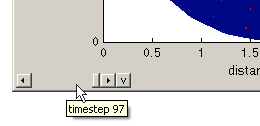
\includegraphics{Ch05/5-9a.png}
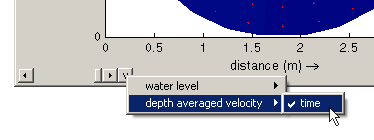
\includegraphics{Ch05/5-9b.png}}
\caption{Slider and object/dimension selection button marked with the character v.}
\label{fig:5.16}
\end{figure}

\section{Animating results} \label{Sec:AnimateResults}
The slider allows you to interactively change between time steps, stations or grid lines.
If you combine these plots together you have an animation.
For this purpose each figure contains an Animation menu; select Start from this menu (or press Ctrl+A).
If there is anything to animate in the figure, a dialog appears as shown in \Fref{fig:5.17}.
The animation will vary the same objects and dimensions as the slider does at the moment that the animation dialog opens.
Therefore, the creation of an animation starts by selecting the object(s) and dimension to animate using the procedure described in the previous section.

The dialog contains six fields.

\begin{itemize}
\item output: The first field allows you to indicate whether you want each picture of the animation written to be stored.
You may select one of the supported bitmap formats (TIF, JPG, PNG or BMP), output via the print/export option (automatically send a series of figures to the printer) or create an AVI file (Windows only).
\item render in background: When creating output (other than to the screen), you can select the option to render in background.
This accelerates the image generation.
This option is not available for BMP files which are created from screen grabs.
\item steps: The second field allows you to select the time steps and spatial co-ordinates that should be part of the animation.
You can walk through the steps in any order you like, e.g. backwards (97:-1:1) or more detailed in one range (1:19 20:5:95).
\item loop until stopped: The last field enables you to animate the selected steps repeatedly until the animation is explicitly stopped.
This option only available if the output option is set to no output.
\item maximum frame rate: Because animations on small datasets and fast hardware may be too fast to follow, you can set a maximum display frame rate.
This frame rate is also used when creating an AVI animation as the frame rate of the animation.
\item script: When you run QUICKPLOT\ as part of the \DMATLAB\ interface from within MATLAB, you may optionally specify an m-file script to run after each plot update.
This allows you to make final adjustments to the plot using MATLAB features.
This option is not available in the standalone \QUICKPLOT\ version.
\end{itemize}

The default setting is to animate the results for the full range of the dimension to be varied (for instance all time steps or all N co-ordinates) without storing the pictures.
Instead of storing the pictures on disk, the program can also copy the files to the clipboard (useful if you have another program that can collect them automatically) or send them to a printer.
The animation can be stopped by pressing Ctrl+H or selecting Stop from the Animation menu.

\begin{figure}
\center{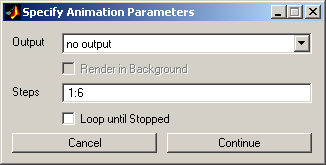
\includegraphics{Ch05/5-10.png}}
\caption{Dialog for the animation settings.}
\label{fig:5.17}
\end{figure}

\begin{Remark}
\item If you are using the animation option for the purpose of creating files (i.e.\ not for immediate viewing), you may generally cover or minimise the figure that is being animated (or select Render in Background).
However, there is one exception: BMP files are created using a screen capture process which will produce undesired effects when the figure playing the animation is not on top.
\item When creating an animation it is generally best to use consistent colouring and scaling for all pictures/frames of the animation.
Set vector scaling, colour thresholds and colour limits manually as indicated in Sections \ref{Sec:VectorScaling}, \ref{Sec:Thresholds} and \ref{Sec:ColourLimits}.
For 1D and 2DV plots, use the zoom option explained in \Sref{Sec:InteractPlot} to keep the plot ranges fixed.
\end{Remark}

\section{Defining and combining variables} \label{Sec:DefVariables}
Sometimes it is useful to determine derived quantities, like minimum, mean or maximum values of some quantities over a (rectangular) part of the domain (e.g.\ a cross-section) or to determine the Froude number in each point.
For these purposes, the program includes basic functionality for defining variables and combining those using simple expressions.

The first step is defining the variables.
The main program window contains one button that has not yet been explained, namely Define Var., and it does as you probably have guessed, lead to the definition of a variable.
The variable will represent the data selection at the moment that the variable was defined.
For instance, in the case shown in \Fref{fig:5.18}, defining a variable now will cause it to represent the last water level in the selected Delft3D communication file.
However, if you check the Time Step -- All checkbox first, the variable will represent the water level field at all 97 time steps.
Careful data selection before defining the variables is important.

\begin{figure}
\center{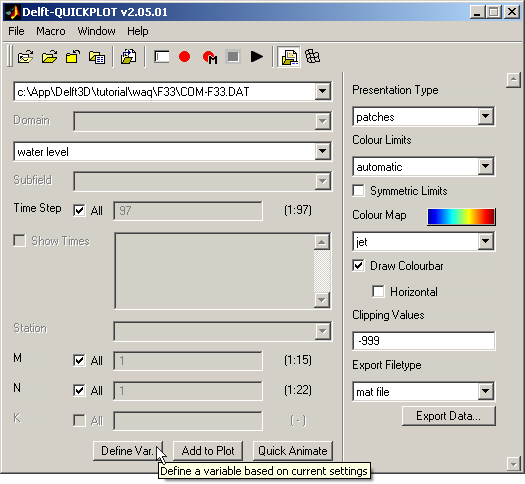
\includegraphics{Ch05/5-11.png}}
\caption{Clicking Define Var.\ will lead to the definition of a variable representing the last water level field in the selected Delft3D communication file.}
\label{fig:5.18}
\end{figure}

Clicking the Define Var.\ button will open a small dialog window requesting a name for the variable (see \Fref{fig:5.19}).
The dialog will persist until you have specified a unique variable name.
Suppose that we define two variables: `water level' and `velocity' representing all 97 water levels and depth averaged velocity fields in the Delft3D communication file used above.

\begin{figure}
\center{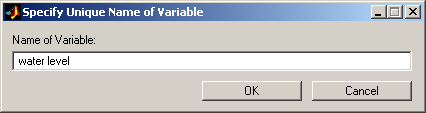
\includegraphics{Ch05/5-12.png}}
\caption{Dialog window requesting a unique name for the variable.}
\label{fig:5.19}
\end{figure}

Once you have defined variables, the label $<$user defined variables$>$ will be available in the list of data files as shown by \Fref{fig:5.20}.
If we select it, the list of data fields will contain the two variables that we had defined: `water level' and `velocity' (see \Fref{fig:5.21}).
It is possible to make plots using these two variables in exactly the same way as the original data fields and all plot and export options still apply.

\begin{figure}
\center{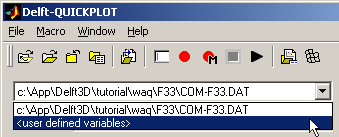
\includegraphics{Ch05/5-13.png}}
\caption{Virtual file labelled $<$user defined variables$>$ in the list of data files.}
\label{fig:5.20}
\end{figure}

\begin{figure}
\center{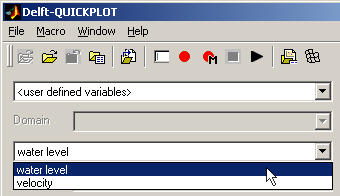
\includegraphics{Ch05/5-14.png}}
\caption{The data field list contains the variables.}
\label{fig:5.21}
\end{figure}

The variables can be manipulated by clicking on the File options button.
The file options dialog for the virtual file $<$user defined variables$>$ allows you to define new variables based on functional relationships of one or two existing variables.
The dialog window is shown in \Fref{fig:5.22}.
The following operators are available:

\begin{itemize}
\item A+B, A-B, A/B, A*B, max(A,B), min(A,B): combine two data sets of compatible size
\item + constant, * constant, \^\ constant, max(A,constant), min(A,constant): combine a data set with a constant
\item 10log, abs: compute logarithm or absolute value of data set
\item magnitude: compute magnitude of vector field
\item series: A,B: treat second variables as a continuation of the first variable (e.g. combine data sets from separate files into one large virtual time-series)
\item A under condition B: use the value of the first variable when the second variable is in a certain range of values.
Acceptable condition statements include a value, e.g.\ 3, a range, e.g.\ [2 3], or all values larger or smaller than a certain value, e.g.\ >3.
See also \Sref{Sec:DefVariables} on clipping data values.
\item max, alg. mean, min, sum of M, N, K: compute maximum, algebraic mean, minimum and sum of a field variable in the indicated grid direction.
The spatial co-ordinates are averaged along the indicated direction.
\end{itemize}

\begin{Remark}
\item Two variables have compatible dimensions if all dimensions (time and space) match for the two variables or if dimensions that do not match are equal to 1 for either one of the variables.
\item The alg.\ mean M, N, K operators compute the algebraic mean and not the weighted average.
For instance, the `alg.\ mean K' operator merely sums all variables in the K direction and divides the sum by the number of points in the vertical, so the computed value does not correspond to the depth averaged value.
\end{Remark}

\begin{figure}
\center{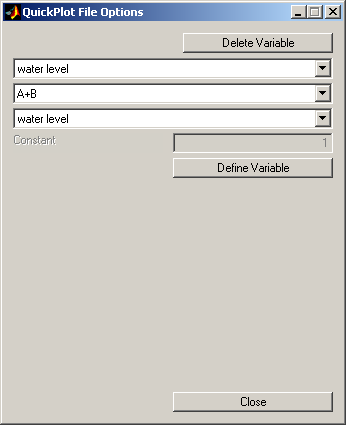
\includegraphics{Ch05/5-15.png}}
\caption{File options dialog window for $<$user defined variables$>$ while defining a new conditional variable.}
\label{fig:5.22}
\end{figure}

Given the operators listed above and the two variables, the Froude number can be defined in five steps assuming a horizontal bed level at 5 m below the reference level:

\begin{enumerate}
\item select the variable `velocity', select operator `magnitude', define a new variable called `magnitude(velocity)'
\item select the variable `water level', select operator `+ constant', specify constant `5', define a new variable `water depth'
\item select the variable `water depth', select operator `* constant', specify constant `9.8', define a new variable `water depth * 9.8'
\item select the variable `water depth * 9.8', select operator `\^\  constant', specify constant `0.5', define a new variable `sqrt(gh)'
\item select the variable `magnitude(velocity)', select operator `A/B', select the variable `sqrt(gh)', define a new variable `Froude'
\end{enumerate}

Switch back to the main program window.
The variable `Froude' and all other intermediate variables are now available for plotting.
Since the original variables, called `water level' and `velocity', were both defined for the whole domain and for all time steps, so is the variable `Froude'.
All plot and export options still apply.

\begin{figure}
\center{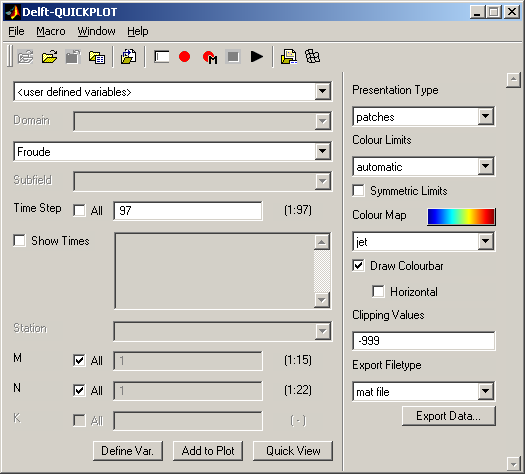
\includegraphics{Ch05/5-16.png}}
\caption{Main program window showing the newly defined variable `Froude'.}
\label{fig:5.23}
\end{figure}

\begin{Remark}
\item The variables are currently self-containing, that is the internal definition of the variable `Froude' contains all information on the intermediate steps and information on the original variables `water level' and `velocity'.
If all other variables are deleted (using the Delete Variable button in the file options dialog) and all files are closed, the `Froude' variable will still be able to plot as long as the files are still in their original location and contain valid data.
Because of reasons of memory efficiency and flexibility, this behaviour is likely to change in a future release.
\end{Remark}

\section{Define your own colour maps} \label{Sec:DefColourMap}
The number of colour maps can be extended interactively by clicking on the preview colour map in the list of plot options as indicated in \Fref{fig:5.24}.

\begin{figure}
\center{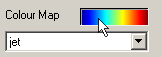
\includegraphics{Ch05/5-17.png}}
\caption{Open the colour map editor by clicking on the colour map preview.}
\label{fig:5.24}
\end{figure}

\begin{figure}
\center{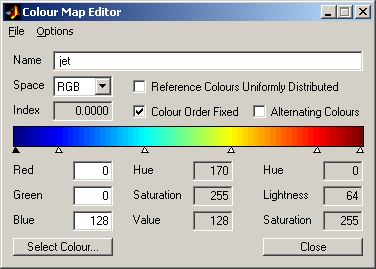
\includegraphics{Ch05/5-18.png}}
\caption{The colour map editor.}
\label{fig:5.25}
\end{figure}

A colour map editor window will open as shown in \Fref{fig:5.25}.
It will initially show the colour map selected in the plot options.
The colours that form the basis of the colour map are indicated by little triangles below the colour bar.
The active colour is indicated by a black triangle whereas the other colours are indicated by white triangles.
Left clicking on the colour bar selects the nearest colour.
Right clicking on the colour map adds a colour at the selected location; the colour will initially match the colour in the original colour map (see \Fref{fig:5.26}).
The colour can be changed by specifying the red, green and blue components (or the resepective components in case of another colour space) or by selecting the colour from a standard colour selection interface (accessible by clicking the Select Colour button in the lower left corner).
The location of the colour on the colour map can be changed by left click and dragging the colour.
Colours can be removed from the colour map by left clicking on them and dragging them away from colour bar.

\begin{figure}
\center{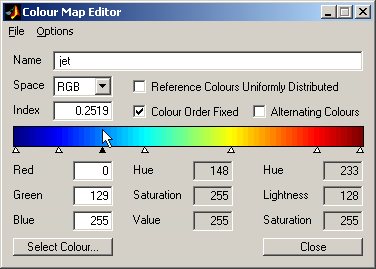
\includegraphics{Ch05/5-19.png}}
\caption{Right click on the colour bar to add a colour.}
\label{fig:5.26}
\end{figure}

When you are satisfied with the new colour map, specify a new name, save it in the colormaps directory as a file with an extension `.clrmap' and close the colour map editor; the new colour will be selected in the main window.
If you don't like the changes don't save the colour map, just press the Close button or open another colour map.

\begin{Remark}
\item Make sure that the colour map has a unique name.
The program will behave incorrectly if there are multiple colour maps with the same name.
Note: the name of the colour map used by \QUICKPLOT\ is the name you specify in the user interface; not the name of the file.
\end{Remark}

\section{Using the Grid View selection window} \label{Sec:GridView}
Besides the Plot Manager described in \Sref{Sec:PlotManager}, you can also start the Grid View selection window from the Window menu of the main program window (command: Open grid view) or from the icon on the toolbar in the same window.
This will open a new window showing a plot of the grid (optionally with grid numbers) in cyan and the selection of the spatial co-ordinates in red as shown in \Fref{fig:5.27} (some of these settings can be changed in the preferences dialog described in \Sref{Sec:GridViewPrefs}).

The interface can be used as an alternative way of selecting a grid line or area to be plotted.
The selection procedure should be started from the Select menu of the Grid View selection window or the associated toolbar button.
There are ten selection options:
\begin{itemize}
\item Grid Point,
\item (whole) Grid Line,
\item Grid Line Segment,
\item Piecewise Grid Line,
\item Shortest Path (by path distance or least number of segments/cells),
\item Arbitrary (x,y) Line,
\item Grid Range,
\item Whole Grid,
\item Arbitrary Rectangle, and
\item Arbitrary Area.
\end{itemize}
Not all selection options are available under all circumstances.
The Shortest Path and Arbitrary Rectangle/Area options are not available for a structured grid, whereas the Grid Line Segment, Piecewise Grid Line, and Grid Range options are not available for an unstructured grid.
The Grid Line option can be used for data defined in cell centres of an unstructured grid if the grid is locally structured.
The Arbitrary (x,y) Line option is available for both structured and unstructured grids, but not for 1D models.
\Fref{fig:5.27} shows a selected Grid Range; \Fref{fig:5.28} shows a General Line while being drawn (the toolbar buttons and menus are disabled while a selection process is ongoing).
A Grid Point is selected using a single click.
A Grid Line is selected using one click to select one point and a second click to select the grid line direction.
A Grid Line Segment is selected by subsequently clicking on the start and end point.
The selection process of Piecewise Grid Line, Shortest Path, Arbitrary Line and Arbitrary Area start and continue with left mouse clicks and finish with a right mouse click.
A Grid Range and Arbitrary Rectangle require two clicks indicating two opposite corners of the range to be selected.
The Whole Grid option does not require any clicks.
The number of options accessible depends on the data set chosen.
During the selection process the mouse co-ordinates are indicated in the lower left corner: both X, Y and M, N co-ordinates.
When the selection process is switched off, you can zoom in by dragging a zoom area while keeping the left mouse button pressed and zoom out by pressing the right mouse button.

\begin{figure}
\center{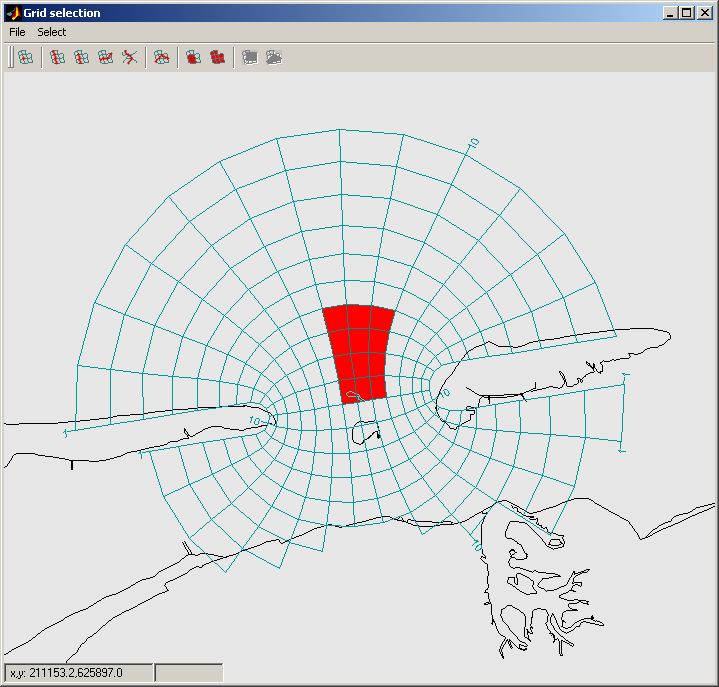
\includegraphics[width=100mm]{Ch05/grid_selection_grid_range.png}}
\caption{Grid View selection window after the selection of a Grid Range.}
\label{fig:5.27}
\end{figure}

\begin{Remark}
\item If the toolbar buttons and menus of the Grid View window are disabled, you're in a selection mode.
To leave the selection mode without completing the selection process, press the Escape Key.
\item Depending upon the type of the data file, the Grid View selection window may either switch between different grid representations depending on the stagger-position of the selected data field in the main program interface, or switch between face/cell, edge or node selection mode.
The former method is currently used for some structured grid data sets whereas the second method has been introduced for unstructured data sets.
\item For large models (re)drawing the Grid View selection window may require a significant amount of time, therefore, it is advised to keep the window closed in general.
\item For reference one can load one or more land boundary files from the File, Show Land Boundary menu in the Grid View window.
These land boundaries will remain to be displayed until you select the File, Show Land Boundary menu item and cancel the selection of a new land boundary file.
Acceptable file formats are Tekal two column landboundary files, BNA files, ArcInfo generate files and polyline Esri shape files.
\end{Remark}

\begin{figure}
\center{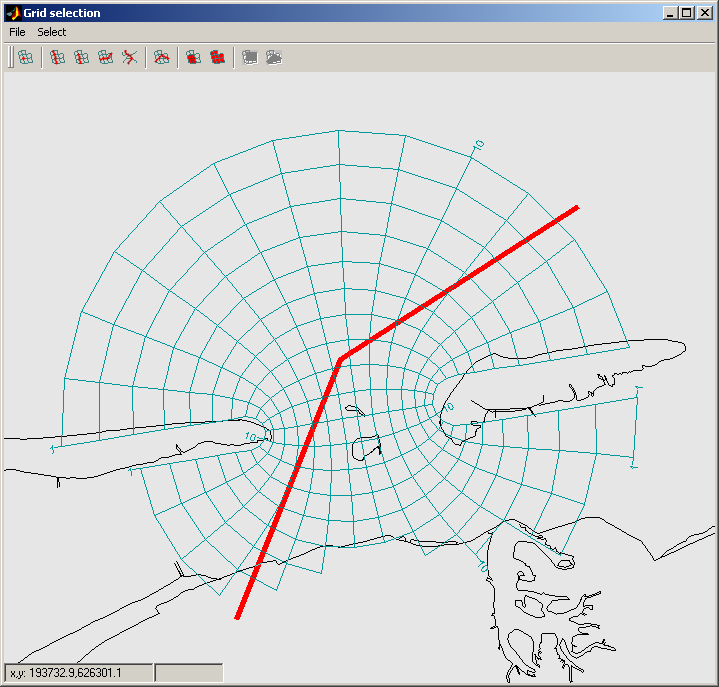
\includegraphics[width=100mm]{Ch05/grid_selection_arbitrary_line}}
\caption{Grid View selection window while selecting an Arbitrary Line.}
\label{fig:5.28}
\end{figure}

\section{Using log files as macros} \label{Sec:Macros}
\QUICKPLOT\ has log file functionality for all actions of the main program window and some secondary interfaces, such as the file options dialog.
This functionality can be accessed from the Macro menu and the macro icons on the toolbar of the main program interface as shown in \Fref{fig:5.29}.

\begin{figure}
\center{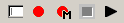
\includegraphics{Ch05/5-21a.png}
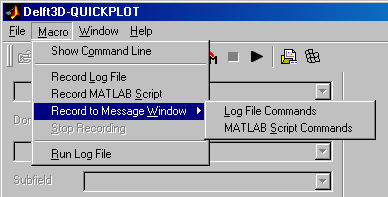
\includegraphics{Ch05/5-21b.png}}
\caption{Logfile icons in the main program interface.}
\label{fig:5.29}
\end{figure}

The icons have (from left to right) the follow purpose:

\begin{itemize}
\item Open the \QUICKPLOT\ command line interface (menu item: Show Command Line).
In general you will not need this, it is used for testing out new functionality.
\item Record commands to a log file (menu item: Record Log File).
\item Record commands to a MATLAB script file (menu item: Record MATLAB Script).
\item Stop recording the commands (menu item: Stop Recording)
\item Play/re-run a log file (menu item: Run Log File).
\end{itemize}

When the recording of commands is started all commands will be written in ASCII format to a file (extension .qplog) specified by you until you stop the recording.
The commands stored in a log file can be played back, that is, log files can be used as macros.
To repeat the list of commands stored in a log file, select the Run Log File option and select the file.
The MATLAB script file is intended for use with the \DMATLAB\ interface, but can be re-run using the Run Log File option as well.

In addition to writing the commands to a log or script file, it is possible to echo the commands to the \QUICKPLOT\ Message Window.

This manual does not explain the commands in the log file.
Below you find an example of the log file of the procedure to define the Froude variable in \Sref{Sec:DefVariables} from the opening of the file until the first plot.

\begin{Verbatim}
openfile 'd:\Delft3D\tutorial\waq\f34\com-f34-waq.dat'
selectfield 'water level'
allt 1
defvariable 'water level'
selectfield 'depth averaged velocity'
defvariable 'velocity'
selectfile '<user defined variables>'
fileoptions 'selectvar' 'velocity'
fileoptions 'selectoperator' 'magnitude'
fileoptions 'defvariable' 'magnitude(velocity)'
fileoptions 'selectvar' 'water level'
fileoptions 'selectoperator' '+ constant'
fileoptions 'const' 5
fileoptions 'defvariable' 'water depth'
fileoptions 'selectoperator' '* constant'
fileoptions 'const' 9.8
fileoptions 'defvariable' 'water depth * 9.8'
fileoptions 'selectoperator' '^\ constant'
fileoptions 'const' 0.5
fileoptions 'defvariable' 'sqrt(gh)'
fileoptions 'selectvar' 'magnitude(velocity)'
fileoptions 'selectoperator' 'A/B'
fileoptions 'selectvar2' 'sqrt(gh)'
fileoptions 'defvariable' 'Froude'
selectfield 'Froude'
allt 0
quickview
\end{Verbatim}

\begin{figure}
\center{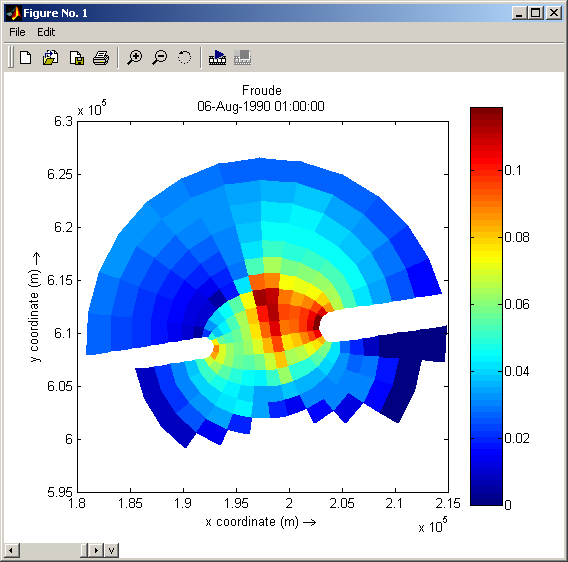
\includegraphics{Ch05/result_matlab_script.png}}
\caption{End result of the example log file and MATLAB script.}
\label{fig:5.30}
\end{figure}

\begin{Remark}
\item Interactive commands (manipulation of plots) are not recorded.
\item As an alternative to a log file, you can write a MATLAB script file.
Its basic syntax is the same, but it consists of valid MATLAB commands to be used in combination with the \DMATLAB\ interface that allows for integration of \QUICKPLOT\ features and the tools of the MATLAB environment.
The equivalent MATLAB script reads:
\end{Remark}

\begin{Verbatim}
d3d_qp('openfile','d:\Delft3D\tutorial\waq\f34\com-f34-waq.dat')
d3d_qp('selectfield','water level')
d3d_qp('allt',1)
d3d_qp('defvariable','water level')
d3d_qp('selectfield','depth averaged velocity')
d3d_qp('defvariable','velocity')
d3d_qp('selectfile','<user defined variables>')
d3d_qp('fileoptions','selectvar','velocity')
d3d_qp('fileoptions','selectoperator','magnitude')
d3d_qp('fileoptions','defvariable','magnitude(velocity)')
d3d_qp('fileoptions','selectvar','water level')
d3d_qp('fileoptions','selectoperator','+ constant')
d3d_qp('fileoptions','const',5)
d3d_qp('fileoptions','defvariable','water depth')
d3d_qp('fileoptions','selectoperator','* constant')
d3d_qp('fileoptions','const',9.8)
d3d_qp('fileoptions','defvariable','water depth * 9.8')
d3d_qp('fileoptions','selectoperator','^\ constant')
d3d_qp('fileoptions','const',0.5)
d3d_qp('fileoptions','defvariable','sqrt(gh)')
d3d_qp('fileoptions','selectvar','magnitude(velocity)')
d3d_qp('fileoptions','selectoperator','A/B')
d3d_qp('fileoptions','selectvar2','sqrt(gh)')
d3d_qp('fileoptions','defvariable','Froude')
d3d_qp('selectfield','Froude')
d3d_qp('allt',0)
d3d_qp('quickview')
\end{Verbatim}
